\documentclass[12pt]{article}
\usepackage[utf8]{inputenc}
\usepackage[left=2.5cm, right=2.5cm, top=2.5cm, bottom=2.5cm]{geometry}
\renewcommand{\thesection}{\Roman{section}}

\newcommand{\HRule}{\rule{\linewidth}{0.5mm}}

\usepackage{wrapfig}

\usepackage{tcolorbox}
\usepackage{diagbox}

\usepackage{indentfirst}
\usepackage{setspace}

\usepackage{graphicx}
\graphicspath{ {./} }

\usepackage{xcolor,colortbl}

\usepackage{fancyhdr}
\pagestyle{fancy}

\setlength{\headheight}{15pt}
\fancyhead[R]{EPITA - Lyon}
\fancyhead[L]{Guardians Studio}
\fancyfoot[CO]{\thepage}
\renewcommand{\baselinestretch}{1.1} 

\renewcommand*\contentsname{Table des matières}

\usepackage{hyperref}

\hypersetup {
    colorlinks,
    citecolor=black,
    filecolor=black,
    linkcolor=black,
    urlcolor=black 
}


\title {
\HRule \\[0.4cm]
    Cahier des charges - Guardians Studio
    \\
    \textbf{Era Of Guardians : Timeless Village}
\HRule \\[1cm]
}




\author {
    Alexandre Privat - Erwann Lesech - Guillaume Jolivalt - Raphaël Heng
}

\date {
    EPITA Lyon $|$ Promo 2026 
}

\begin{document}
    
    \maketitle
    \begin{figure}[h]
    
\includegraphics[width = 10cm, height = 10cm]{Logo.png}
    \centering
    \end{figure}
    \clearpage
    \tableofcontents
    \clearpage
    
    \section{Introduction}
        Durant ces dernières années, les jeux multijoueurs qui se sont imposés furent les jeux de tirs ou les MOBA ("multiplayer online battle arena" en anglais ou "arène de bataille en ligne multijoueur" en français). Or, notre groupe "Guardians Studio" se veut gardien du plaisir de jeu pour chacune et chacun. C'est pourquoi notre projet, sous forme d'un jeu, consistera en une aventure scénarisée coopérative pour que tous les joueurs puissent vivre une expérience immersive et plaisante tout en renforçant leurs liens.
        \\
       \par\textbf {Era Of Guardians : Timeless Village} est donc un RPG (Role Playing Game) scénarisé en 3D à la vue première personne dans lequel le joueur aura pour objectif de compléter des quêtes dans l'univers d'Astria afin de ramener à la vie \textbf{Tidalar le Gardien}, pour rendre aux habitants d'Hazeltown le cours du temps qui dès lors s'était interrompu.
       \\
       \par Ce projet, développé dans le cadre de notre semestre 2 à l'EPITA, est édité par notre groupe : \textbf{Guardians Studio} sous le moteur de jeu \textbf{Unity} utilisant principalement le langage \textbf{C\#}.
       \\
       

        \subsection{Guardians Studio}
        Notre groupe : le \textbf{Guardians Studio} a pris forme au cours de nos révisions d'examens de mi-semestre durant lesquelles nous avons su nous aider les uns les autres en fonction de nos facilités et difficultés. Désirant alors une équipe soudée et capable d'entraide au cours de ce projet majeur, nous avons décidé de former le "Guardians Studio" (traduit : Studio des Gardiens). 
        \\
        
        \subsection{Création du logo}
        
            La première étape dans le processus de création du logo a été de faire des croquis sur papier. Nous avons ensuite, utilisé un logiciel de vectorisation d'image afin d'obtenir une qualité sans perte lors de l'ajout du logo. En effet, l'exportation d'image à de nombreuses reprises, avec des logiciels de retouche photographique, détériore grandement la qualité de l'image et cela se ressent sur le résultat final de notre logo.
            \\
            \par Nous avons créé ce logo comme prolongement de l'idée de notre jeu. En effet, il est composé d'un casque d'un temps passé sur lequel des gemmes sont posées ; ces gemmes étant celles que nous devons ramasser dans notre jeu. Par ailleurs, le nom du studio est écrit en utilisant une typologie très moderne ce qui crée un contraste temporel entre le vieux casque et la police plutôt moderne ; le temps étant un sujet proéminent dans notre jeu.
        
        
        \subsection{Présentation de l'équipe}
        \hfill
            \begin{tcolorbox} [
                coltitle=black, 
                colframe=blue!20!white, 
                colback=blue!5, 
                title=\subsubsection{Raphaël "Noton" Heng (Chef de projet)}
            ]
                
                \setlength{\parindent}{3ex} 
                \textbf{Amateur de vidéo du groupe}, j'ai commencé à programmer dès l'année de Seconde avec l'enseignement d'exploration \textit{Informatique \& Création Numérique}. J'y ai découvert des bases de Python, de HTML et de CSS. 
                \\
                \par Ce projet est une opportunité pour moi d'approfondir mes connaissances en développement, en production de vidéo et en modélisation.
            \end{tcolorbox}
            \begin{tcolorbox} [
                coltitle=black, 
                colframe=green!40!white, 
                colback=green!5, 
                title= \subsubsection{Alexandre "Zeflash" Privat (Responsable scénario)}
            ]

            \setlength{\parindent}{3ex} \textbf{Fan de casse tête et de réflexion}, j'ai découvert la programmation en classe de première, ma curiosité de découvrir différents langages informatiques et de découvrir la composition d'une machine m'a motivé à me lancer dans une branche de l'ingénierie informatique.
            \\
            \par Ce projet de réaliser un jeu me permettra d'apprendre de nouvelles choses et d'avoir une autre vision des jeux vidéo.
            
            \end{tcolorbox}
            
            \begin{tcolorbox} [
                coltitle=black, 
                colframe=orange!50!white,
                colback=orange!5,
                title= \subsubsection{Erwann "R-One" Lesech (Responsable Réseau)}
            ]
                \setlength{\parindent}{3ex} \textbf{Roux et motard du groupe}, sportif originaire du sud, j'ai découvert le développement informatique il y a 4 ans. J'ai été amené à coder différents petits jeux et applications sans grandes ambitions. 
                \\
                \par Ce projet de 6 mois par groupe de 4 est une opportunité passionnante qui je l'espère me permettra d'en apprendre beaucoup sur la gestion d'un projet en groupe, les systèmes réseaux ou encore les intelligences artificielles.
            \end{tcolorbox}
            
            \begin{tcolorbox} [
                coltitle=black, 
                colframe=purple!40!white, 
                colback=purple!10, 
                title= \subsubsection{Guillaume "Guimauve" Jolivalt (Responsable Modélisation)}
            ]
                \setlength{\parindent}{3ex} \textbf{Curieux}, je m'intéresse à beaucoup de domaines de la programmation et de l'informatique depuis bien longtemps. Je n'ai malgré cela encore jamais entrepris de projet aussi conséquent que celui ci. 
                \\
                \par Ce projet est un moyen parfait pour s'essayer à différents aspects dans la création d'un jeu qui m'intéressent tous autant les uns que les autres.
            \end{tcolorbox}

    \section{Era Of Guardians : Timeless Village}
        \subsection{Fondations du jeu}
            \subsubsection{Concepts et intérêts}
                \textbf{Era Of Guardians : Timeless Village} est un RPG (Role Playing Game) qui se joue seul ou en coopération. L'équipe de joueur est amenée, à travers une aventure scénarisée, à évoluer dans différents biomes (macroécosystèmes) pour récupérer 4 gemmes et combattre le Gardien du Temps afin de rétablir le court du temps qui s'est interrompu dans le village d'Hazeltown.
                \\
                \par Ce jeu 3D se jouant à la vue première personne permettra au groupe d'apprendre à se servir du moteur de jeu Unity, d'implémenter un système multijoueur et d'intelligence artificielle pour le comportement des ennemis mais surtout apprendre à s'organiser pour mener à bien ce projet de groupe.
                \\
                
            \subsubsection{Origine du projet}
                Notre groupe étant composé d'amateurs de jeux vidéo en ligne, nous avons pensé qu'il serait intéressant de divertir en cette période de crise sanitaire. Ainsi nous avons choisi de développer un jeu vidéo en utilisant notre expérience.
                \\
                \par Nous avons réfléchi pendant plusieurs jours pour trouver le projet idéal à développer liant multijoueur, I.A. mais aussi level design, gestion de quêtes, utilisation de consommables, combat, ambiance sonore et visuels.
                \\
                \par C'est lors de notre \textbf{quatrième} soirée que nous avons eu l'idée de développer un jeu à monde semi-ouvert ou les joueurs évolueraient en coopération dans plusieurs environnements, nous poussant à apprendre toujours plus de méthodes afin de modéliser de multiples éléments différents.
            
                \clearpage
                
            \subsubsection{Inspirations - Etude de l'art}
                
                \textbf{Le premier jeu vidéo RPG} est \textit{Dungeons and Dragons}, développé par Gary Whisenhunt et Ray Wood en 1975 sur le système \textit{PLATO à l’université du Sud de l'Illinois à Carbondale}.
                \par Dans ce jeu, le joueur doit créer un personnage et s'aventurer dans diverses niveaux à la recherche de trésors. Des monstres peuplent les souterrains et lorsque le joueur récupère "L'Orbe" et réussit à revenir à la surface, son nom est signalé à tous les autres.
                \\
                 \begin{figure}[h]
                    \centering
                    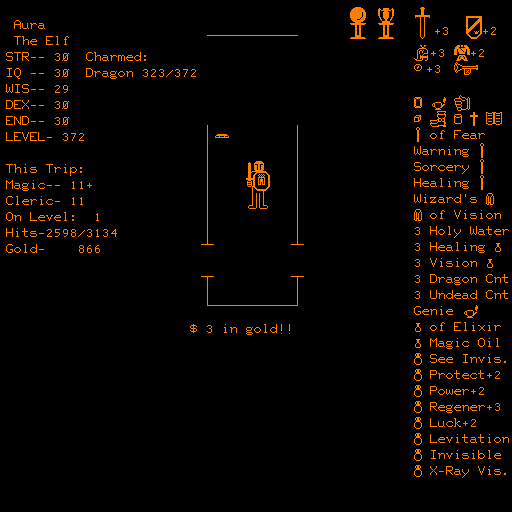
\includegraphics[width=16cm, height=9cm]{Dnd8won.png}
                    \caption{Dungeons and Dragons}
                \end{figure}
                \\
                \par Nous pouvons citer d'autres exemples de RPG comme la série des \textit{The Legend Of Zelda}
                où l'objectif du jeu est de s'aventurer dans le royaume d'Hyrule et de le sauver des forces du mal ou encore la série des \textit{Assassin's Creed} du studio \textit{Ubisoft} qui sont des aventures RPG où le joueur est plongé à travers des évènement passés.
                
                \clearpage

                \par Il existe aussi la série des \textit{Resident Evil}, des \textbf{RPG Horror}, dont le but est généralement d'evoluer dans un environnement dramatique suivant un scénario du même genre. 
                \\On s'inspire notamment de leur manière de gérer la \textbf{"World Map"}.
                \\
                \begin{figure}[h]
                    \centering
                    \includegraphics[width=16cm, height=10cm]{Carte_du_village.png}
                    \caption{Carte de Resident Evil : Village}
                \end{figure}
                \\
                \par Et pour finir, notre jeu s'inspire d'un RPG gratuit nommé \textit{Genshin Impact}, ce dernier est lui-même très inspiré de \textit{The Legend Of Zelda: Breath Of The Wild} et mélange aventure, monde ouvert et maîtrise de différents éléments tels que \textbf{le feu}, \textbf{l'eau}, \textbf{la foudre}, \textbf{le vent}, \textbf{la terre} et \textbf{la glace}. 

                \par Dans ce jeu, il est possible de jouer jusqu'à 4 sur le monde d'un joueur et nous sont offerts la possibilité de défier de puissants ennemis, d'explorer certaines zones et faire des quêtes, le tout en coopération.
                \\
                \par Ces jeux se démarquent par leurs diverses qualités ; ils sont en effet caractérisés par un monde ouvert mais également par leurs nombreuses possibilités de "Gameplay" ainsi qu'un scénario prenant.
                \clearpage

        \subsection{Éléments du jeu}
            \subsubsection{Scénario}
    
                Nous avons le profond désir de faire voyager tous les joueurs durant leur session de jeu. Pour ce faire, quoi de mieux qu'un scénario immersif mêlant intérêt, suspens et réflexion :
                \\
                \par 
                \textit{Dans des temps anciens, les humains ont pendant des siècles, dominé les autres civilisations d'\textbf{Astria}, région de pseudo-cohabitation.Ces dernières, lasses de ces injustices se sont réunies afin de se venger. Unis contre leur ennemi commun, ils firent tomber \textbf{Tidalar}, le Gardien du Temps d'\textbf{Hazeltown}}.
                \\

                
                \par 
                \textit {
                    Plongé alors dans un long sommeil, seul un guerrier appelé par l'esprit des gemmes temporelles bravera forêts, monts et marées pour ainsi accomplir sa quête}.
                \\

                \par 
                \textit {
                    Une fois cela fait, il devra réveiller \textbf{Tidalar} pour que le temps reprenne son cours. Cependant, il devra, avant cela, raisonner le Gardien, désemparé après cette bataille sanglante}.
                
                

            \subsubsection{Principes fondamentaux}
            
                Era Of Guardians : Timeless Village consiste en une équipe de 1 à 4 joueurs qui doit compléter des quêtes en combattant des ennemis (qui sont des I.A.) afin d'améliorer ses capacités tout au long du scénario avec lesquelles elle devra vaincre un boss final. 
                \par Ces joueurs verront leurs statistiques singulières s'améliorer au cours de l'aventure par acquisition de points d'expériences obtenu pour avoir vaincu des ennemis ou encore complété des quêtes. En effet, le scénario n'est pas exclusivement tourné vers un unique objectif. Les difficultés mineures que rencontrent les différents autochtones d'Astria pendant ce drame peuvent être résolues par les joueurs (voir section quêtes).
                
                On essaiera d'implémenter une fonctionnalité de sauvegarde automatique ainsi qu'un système de classes a leur disposition qui auront chacune leurs spécificités. (voir section Bonus)
                
                Dans un objectif de rejouabilité, nous allons limiter le temps de l'aventure permettant le Speedrun, le principe étant de finir le jeu le plus vite possible.
        \clearpage
            \subsubsection{Environnement de jeu}
            
                Les joueurs évolueront dans une ambiance fantaisiste due en partie au scénario du même genre. Ils devront alors voyager à travers 5 macroécosystèmes :
                \begin{itemize} 
                    \setlength{\itemindent}{2em}
                    \item \textbf{Le village d'Hazeltown}, qui est la zone centrale du jeu ou le joueur repasse poser les différentes gemmes.
                    \item \textbf{La forêt de Langdale}
                    \item \textbf{Le Mont Celtia}
                    \item \textbf{L'Okeanos}
                    \item \textbf{Le volcan Turon}
                \end{itemize}

            \subsubsection{Personnages}
                
                Concernant les mouvements, chaque personnage pourra courir, sauter, courir sur les murs et "dasher"(faire une vive accélération dans une direction). Ces aptitudes pourront être acquises au cours de l'aventure.
                \par De plus, en fonction de ses armes, il pourra attaquer et se défendre.
                Dès le lancement d'une compétence, un compte à rebours se déclenchera durant lequel il ne pourra pas relancer une compétence (voir Menus et interfaces).
                \\
                \par Pour comprendre toutes ces mécaniques, notre jeu débutera par un tutoriel qui en plus d'introduire les différentes fonctionnalités, marquera le début du scénario.
                
            \subsubsection{Réseau \& multijoueur}
                Nous avons le profond désir de pouvoir jouer de façon coopérative à \textbf{EOG : Timeless Village}. Pour ce faire, nous allons implémenter un Photon Unity Networking (PUN) afin que les joueurs se retrouvent dans les mêmes instances de jeu.
                
                \par Cela permettra à chaque joueur de visualiser les actions de ses coéquipier et ainsi de s'entraider pour avancer dans l'aventure.
            
            \subsubsection{Ennemis/Intelligence Artificielle}
                On distingue deux types de routines fonctionnant par intelligence artificelle :
                    \\ Une passive, les ennemis se déplaceront dans une zone donnée dans laquelle des éléments extérieurs peuvent altérer leur comportement comme par exemple du bruit suspects.
                    \\ Une active, les ennemis enclenchent un combat et nous ferons en sorte qu'ils attaquent lorsqu'on s'approche trop d'eux et qu'ils réagissent faces aux assauts des joueurs.
                \\
                \par Quant au Gardien, nous ferons en sorte qu'il ait des attaques différentes selon notre position dans la zone de combat et son état.
        \clearpage
            \subsubsection{Quêtes et consommables}
            
                Dans une volonté d'immersion au sein de notre univers, nous allons encourager les joueurs à réaliser des tâches en parlant aux personnages non-joueurs, ils seront amenés à voyager dans divers environnements pour aller livrer des messages, chercher un butin, éliminer une entité malveillante. Tout cela afin d'obtenir des objets afin d'accomplir leur quête principale.
                \\
                \par Après avoir réalisé les quêtes secondaires, les joueurs obtiendront des objets afin d'améliorer les caractéristiques de leur personnage et leurs compétences de combat.
                Les quêtes permettront également d'en apprendre davantage sur l'univers du jeu avec par exemple des parchemins. Les consommables seront utilisables en combat pour aider les joueurs.
            
            \subsubsection{Menus et interfaces}
            
                Nous allons implémenter plusieurs menus :
                    \begin{itemize}
                        \setlength{\itemindent}{2em}
                        \item Menu principal 
                    \end{itemize}
                    \begin{figure}[ht]
                        \centering
                        \includegraphics[width=17cm, height=9cm]{"MainMenu (2).png"}
                        \textbf{\caption{Arborescence des menus principaux}}
                        \label{fig:Menu}
                    \end{figure}
                        
                    \begin{itemize}
                        \setlength{\itemindent}{2em}
                        \item Menu "Pause"
                        \item Inventaire
                        \item Carte (indique la zone où se situe le joueur)
                        \item Menu quêtes
                    \end{itemize}
                    
                 \clearpage
                    
                L'interface joueur sera composée des informations suivantes :
                   \begin{itemize}
                        \setlength{\itemindent}{2em}

                       \item Barre de vie
                       \item Cooldown, compétences
                       \item Barre d'expérience
                       \item (Bonus) Boussole et localisation
                   \end{itemize}
                   \begin{figure}[ht]
                            \centering
                             \includegraphics[width=17cm, height=9cm]{"UI.png"}
                            \textbf{\caption{Croquis d'un ATH (interface joueur) envisageable}}
                            \label{fig:ATH}
                        \end{figure}
                        
            \subsubsection{Ambiance sonore et visuelle}
                Nous utiliserons plusieurs musiques :
                \begin{itemize}
                    \setlength{\itemindent}{2em}

                    \item Thème principal par biomes
                    \item Musiques de "boss"
                \end{itemize}
                \par et des effets sonores sur les armes et les compétences.
                \\
                \par Afin d'introduire le scénario, nous utiliserons des voix-off ainsi que des cinématiques pour faire comprendre aux joueurs le contexte de leur aventure et leur indiquer le fil conducteur afin qu'ils ne s'y perdent pas.
                \\
                
                \par Parallèlement, chaque entrée dans une zone s'accompagnera d'une cinématique de présentation de la zone et de ses points d'intérêts majeurs. 
            
            \subsubsection{Bonus}
                Cette section présente les éléments que nous allons implémenter "Si le temps nous le permet"; en effet, n'ayant guère d'expérience, nous préférons proposer des éléments à développer à terme si tous ce qui a été énoncé ci-dessus a déjà été mis en place.
                \\
                \par \textbf{Personnages} : il y aura 4 classes de personnages jouables afin d'augmenter les possibilités de combinaisons en multijoueur.
                \begin{enumerate}
                \setlength{\itemindent}{2em}
                    \item Corps à corps
                    \begin{itemize}
                        \item Berserk
                        \item Épéiste
                    \end{itemize}
                    \item Distance
                    \begin{itemize}
                        \item Mage
                        \item Archer
                    \end{itemize}
                \end{enumerate} 
                
                \par \textbf{Sauvegarde} : Implémenter un système de sauvegarde automatique à chaque fois qu'une zone est terminée en plus des sauvegardes faites par le joueur manuellement.
                Ces sauvegardes seront enregistrés localement.
                \\
                \par \textbf{Boss} : Implémenter un mini boss par région pour signer la fin de toutes les quêtes faite par les joueurs dans la région.
                \\
                \par \textbf{Multijoueur} : Proposer des "énigmes" dans les différents biomes où la présence de plusieurs joueurs est obligatoire pour réussir à les compléter.
                \\
                
        \subsection{Communication sur le projet}
        
            \subsubsection{Etude de marché}
                Qu'il s'agisse de venir tester notre jeu en cours de développement ou y jouer lorsqu'il sera abouti, nous avons besoin de faire connaître notre jeu vidéo. Tout d'abord, nous nous sommes posés la question de savoir quels étaient les profils qui seraient les plus à même d'être intéresser par ce genre de jeu vidéo. 
                \par Nous en avons conclu que la tranche d'âge des personnes propices était de 15 à 40 ans.
            \clearpage
            \subsubsection{Réseaux sociaux} 
               Pour toucher ce public, il serait préférable de communiquer sur les réseaux sociaux. C'est pourquoi nous ouvrirons un compte sur le réseau "Instagram" sur lequel nous posterons nombres de nos avancés sous forme de courtes vidéos "making-off", d'images attrayantes ou de trailers finaux avec les liens de téléchargement du jeu et du site Web.
            
            \subsubsection{Site Web}
                Nous utiliserons les langages HTML, CSS et JavaScript pour concevoir les différentes pages Web.
                Notre site sera hébergé sur Github Pages et comportera une présentation du groupe ainsi que de ses membres. 
                \\
                Il comportera aussi des liens de téléchargement des différents rapports de soutenances, la chronologie de développement avec les difficultés rencontrées, des vidéos d'aperçu du jeu sans oublier le téléchargement du jeu en lui-même.
        
            
        \subsection{Aspects économiques}
                Lors de nos recherches dans les différents domaines qui nous sont utiles et nécessaires à la création de notre jeu, nous avons découvert que certains aspects du jeu pouvaient engendrer des coûts supplémentaires de développement. Nous nous sommes donc renseignés pour minimiser un maximum ses coûts.
                \\
                \par Tout d'abord, pour héberger le site Web que nous allons créer pour le jeu, nous allons simplement l'hébergeur Github Pages, qui est gratuit. Par ailleurs, pour avoir des serveurs dédiés pour le multijoueur, nous utiliserons les services de Photon Unity Networking (PUN) qui nous permettent d'accueillir bien assez de joueurs sans frais. Enfin, pour ce qui est des assets de modélisation, nous allons les faire nous même ou en prendre quelques uns via l'Asset Store de Unity.
                \\
                \par Ainsi pour ce projet, nous ne pensons pas requérir de quelconques financements. Nous nous fixons du moins l'objectif de ne pas en avoir la nécessité. Nous faisons ce projet dans un but non lucratif, les éventuels bénéfices ne proviendront que des dons de joueurs satisfaits par l'état du jeu.
        \clearpage
        
        \section{Réalisation du projet}
            \subsection{Répartition des tâches}
            
                \begin{table}[ht]
                    \centering
                    \begin{tabular}{|l||*{4}{c|}}
                        \hline
                        \backslashbox[60mm]{\textbf{Tâches}}{\textbf{Membres}} &
                        \textbf{Alexandre} &
                        \textbf{Erwann} &
                        \textbf{Guillaume} &
                        \textbf{Raphaël} 
                        \\
                        
                        \hline
                        \rowcolor{lightgray} \multicolumn{5}{|l|}{\textbf{Infrastructure réseau}}
                        \\
                        
                        \hline
                        \textbf{Multijoueur} & & \cellcolor{red!50} R & & \cellcolor{cyan!60} S
                        \\
                        
                        \hline
                        \rowcolor{lightgray} \multicolumn{5}{|l|}{\textbf{Intelligence Artificielle}}
                        \\
                    
                        \hline
                        \textbf{Routines ennemis} & \cellcolor{cyan!60} S  & & & \cellcolor{red!50} R
                        \\
                        
                        \hline
                        \textbf{IA combat} & & \cellcolor{cyan!60} S & & \cellcolor{red!50} R
                        \\
                        
                        \hline
                        \rowcolor{lightgray} \multicolumn{5}{|l|}{\textbf{Environnement de jeu}}
                        \\
                        
                        \hline
                        \textbf{Terrains} & & & \cellcolor{cyan!60} S & \cellcolor{red!50} R
                        \\
                        
                        \hline
                        \textbf{Modélisation 3D} & & & \cellcolor{red!50} R & \cellcolor{cyan!60} S 
                        \\
                        
                        \hline
                        \textbf{Scénario} & \cellcolor{red!50} R &  \cellcolor{cyan!60} S & & 
                        \\
                        
                        \hline
                        \textbf{Sound Design} & & & \cellcolor{red!50} R & \cellcolor{cyan!60} S
                        \\
                        
                        \hline
                        \rowcolor{lightgray} \multicolumn{5}{|l|}{\textbf{Gameplay}}
                        \\
                        
                        \hline
                        \textbf{Joueur} & & \cellcolor{red!50} R & \cellcolor{cyan!60} S &
                        \\
                        
                        \hline
                        \textbf{Quêtes \& consommables} & \cellcolor{red!50} R & \cellcolor{cyan!60} S & &
                        \\
                        
                        \hline
                        \rowcolor{lightgray} \multicolumn{5}{|l|}{\textbf{Interface}}
                        \\
                        
                        \hline
                        \textbf{HUD} & \cellcolor{cyan!60} S & \cellcolor{red!50} R & &
                        \\
                        
                        \hline
                        \textbf{Menus} & \cellcolor{red!50} R & & \cellcolor{cyan!60} S &
                        \\
                        
                        \hline
                        \textbf{Cinématiques \& trailers} & & & \cellcolor{cyan!60} S & \cellcolor{red!50} R
                        \\
                        
                        \hline
                        \textbf{Installateur} & \cellcolor{cyan!60} S & & \cellcolor{red!50} R & 
                        \\
                        
                        \hline
                        \rowcolor{lightgray} \multicolumn{5}{|l|}{\textbf{Communication}}
                        \\
                        
                        \hline
                        \textbf{Site web} & \cellcolor{cyan!60} S & \cellcolor{red!50} R & & 
                        \\
                        
                        \hline
                        \textbf{Logo} & & & \cellcolor{red!50} R & \cellcolor{cyan!60} S
                       
                        \\
                        \hline
                    \end{tabular}
                    \caption{\textbf{Tableau de la répartition des tâches}, R = Responsable \& S = Suppléant}
                \end{table}
                
                \par Étant un groupe soudé composé de personnes ayant différentes connaissances et préférences, nous avons organisé une répartition des tâches plutôt équilibrée. Elle permet d'assigner un responsable pour chaque tâche et un suppléant qui sera là pour l'épauler. Bien sûr, si une personne a besoin d'aider, toute l'équipe sera à sa disposition pour essayer de venir à bout du problème.
                
                \clearpage
        \subsection{Planification des tâches}
            \begin{table}[ht]
            \centering
                \begin{tabular}{|l||*{3}{c|}}
                    \hline
                    \diagbox{\textbf{Tâches}}{\textbf{Soutenances}} &
                    \textbf{soutenance 1} &
                    \textbf{soutenance 2} &
                    \textbf{soutenance 3} 
                    \\ 
                    \hline
                    \rowcolor{lightgray} \multicolumn{4}{|l|}{\textbf{Infrastructure réseau}}
                    \\
                    
                    \hline
                     \textbf{Multijoueur} & 50\% & 80\% & 100\%
                    \\
                    
                    \hline
                    \rowcolor{lightgray} \multicolumn{4}{|l|}{\textbf{Intelligence Artificielle}}
                    \\
                    
                    \hline
                     \textbf{Routine ennemies} & 20\% & 60\% & 100\%
                    \\
                    
                    \hline
                     \textbf{IA combat} & 25\% & 66\% & 100\%
                    \\
                    
                    \hline
                     \rowcolor{lightgray} \multicolumn{4}{|l|}{\textbf{Environnement de jeu}}
                    \\
                    
                    \hline
                    \textbf{Terrains} & 33\% & 66\% & 100\% 
                    \\
                    
                    \hline
                    \textbf{Modélisation 3D} & 33\% & 70\% & 100\%
                    \\
                    
                    \hline
                    \textbf{Scénario} & 30\% & 60\% & 100\%
                    \\
                    
                    \hline
                    \textbf{Sound Design} & 10\% & 70\% & 100\%
                    \\
                    
                    \hline
                    \rowcolor{lightgray} \multicolumn{4}{|l|}{\textbf{Gameplay}}
                    \\
                    
                    \hline
                    \textbf{Joueur} & 60\% & 80\% & 100\%
                    \\
                    
                    \hline
                    \textbf{Quêtes et consommables} & 20\% & 60\% & 100\%
                    \\
                    
                    \hline
                    \rowcolor{lightgray} \multicolumn{4}{|l|}{\textbf{Interface}}
                    \\
                    
                    \hline
                    \textbf{HUD} & 40\% & 80\% & 100\%
                    \\
                    
                    \hline
                    \textbf{Menus} & 20\% & 60\% & 100\%
                    \\
                    
                    \hline
                    \textbf{Cinématiques et trailers} & 10\% & 50\% & 100\%
                    \\
                    \hline
                    \textbf{Installateur} & 0\% & 10\% & 100\%
                    \\
                    
                    \hline
                    \rowcolor{lightgray} \multicolumn{4}{|l|}{\textbf{Communication}}
                    \\
                    
                    \hline
                    \textbf{Site web} & 10\% & 80\% & 100\%
                    \\
                    
                    \hline
                    \textbf{Logo} & 80\% & 100\% & 100\%
                   
                    \\
                    \hline
                    
                \end{tabular}
                \caption{\textbf{Estimation des avancées des différentes tâches}}
            \end{table}
        \subsection{Moyens matériels}
        
            \par Pour ce jeu vidéo, nous utiliserons des ordinateurs fixes et portables et un serveur pour le multijoueur.
            \par A titre d'indication, voici nos quatre configurations respectives avec lesquelles nous développerons ce jeu :
            
             \begin{enumerate}
                 \item Raphaël Heng
                    \begin{itemize}
                        \item Processeur : AMD Ryzen 7 2700X
                        \item Carte Graphique : AMD Radeon RX 5600 XT
                        \item RAM : 16 Go
                    \end{itemize}
                \clearpage
                \item Erwann Lesech
                    \begin{itemize}
                        \item Processeur : AMD Ryzen 7 5800H
                        \item Carte Graphique : Nvidia RTX 3060
                        \item RAM : 16 Go
                    \end{itemize}
                    
                \item Guillaume Jolivalt
                    \begin{itemize}
                        \item Processeur : Intel Core i7-8700
                        \item Carte Graphique : Nvidia GTX 1060
                        \item RAM : 16 Go
                    \end{itemize}
                
                \item Alexandre Privat
                    \begin{itemize}
                        \item Processeur : Intel Core i7-9750
                        \item Carte Graphique : Nvidia GTX 1650
                        \item RAM : 16 Go
                    \end{itemize}
                    
             \end{enumerate}
                    
        \subsection{Moyens intellectuels}
         Pour ce projet nous utiliserons divers outils tels que :
         
            \begin{itemize}
                \setlength{\itemindent}{2em}
                \item \textbf{Unity}, moteur de jeu en C\#.
                \item \textbf{Visual Studio}, IDE pour développer en C\#.
                \item \textbf{HTML, CSS, PHP, Javascript}, Langages pour la création d'un site web.
                \item \textbf{Davinci Resolve}, logiciel de montage pour monter le trailer.
                \item \textbf{Mixamo}, logiciel d'animation pour nos personnages.
                \item \textbf{Blender}, logiciel de modélisation 3D.
                \item \textbf{Davinci Resolve ou After Effects}, logiciel d'effet spéciaux et de compositing.
                \item \textbf{Inkscape}, pour le logo.
            \end{itemize}
        

    \section{Conclusion}
        Pour conclure, ce projet consiste en la réalisation d'un jeu vidéo en C\# à l'aide du moteur de jeu Unity. Chaque membre du groupe s'est vu attribué un nombre d'ajouts à implémenter dans le jeu en fonction de ses capacités et envies. Il s'agit pour nous tous d'une première expérience en terme de développement sur 6 mois et par groupe de 4 personnes. C'est un projet très ambitieux pour notre niveau, c'est donc pour cette raison que nous allons redoubler d'efforts afin de pouvoir proposer, en juin, un produit fini de qualité.
    
\end{document}
